\documentclass{beamer}
\usepackage{amsfonts,amsmath,oldgerm,graphicx,epstopdf}
\usepackage{booktabs}
\epstopdfsetup{outdir=illustration/}
\setbeamertemplate{caption}{\color{maincolor}Fig. \color{darkgray} \raggedright\insertcaption\par}

\usetheme{sintef}

% \newcommand{\testcolor}[1]{\colorbox{#1}{\textcolor{#1}{test}}~\texttt{#1}}

\usefonttheme[onlymath]{serif}

\titlebackground*{assets/background}

\newcommand{\hrefcol}[2]{\textcolor{cyan}{\href{#1}{#2}}}

% TODO: aggiornare titolo, aggiungere corelatore.

\title{\large{Investigation of the synthesis of a new pyrazole dicarboxylate ligand for the construction of new MOFs}}
\course{\vspace{0.2cm}\tiny Relatrice: Prof. Lucia Carlucci \\ \vspace{-0.2cm} Co-relatore: Pierluigi Mercandelli}
\subtitle{Laurea Triennale in Chimica}
\author{\href{stefano.marton@studenti.unimi.it}{Stefano Marton}}
\IDnumber{962848}

\begin{document}
\maketitle

\section{Sintesi del legante pirazolico}

\setlength{\columnsep}{0.2cm}
\begin{frame}{Perché leganti con funzionitá pirazoliche?}
	\begin{columns}
		\hspace{1cm}
		\begin{column}{0.3\textwidth}
			\begin{itemize}
				\item Affinitá con Al
				\item Legami idrogeno
				\item Rigiditá strutturale
			\end{itemize}
		\end{column}
		\hspace{-1cm}
		\begin{column}{0.7\textwidth}
			\begin{figure}[h]
				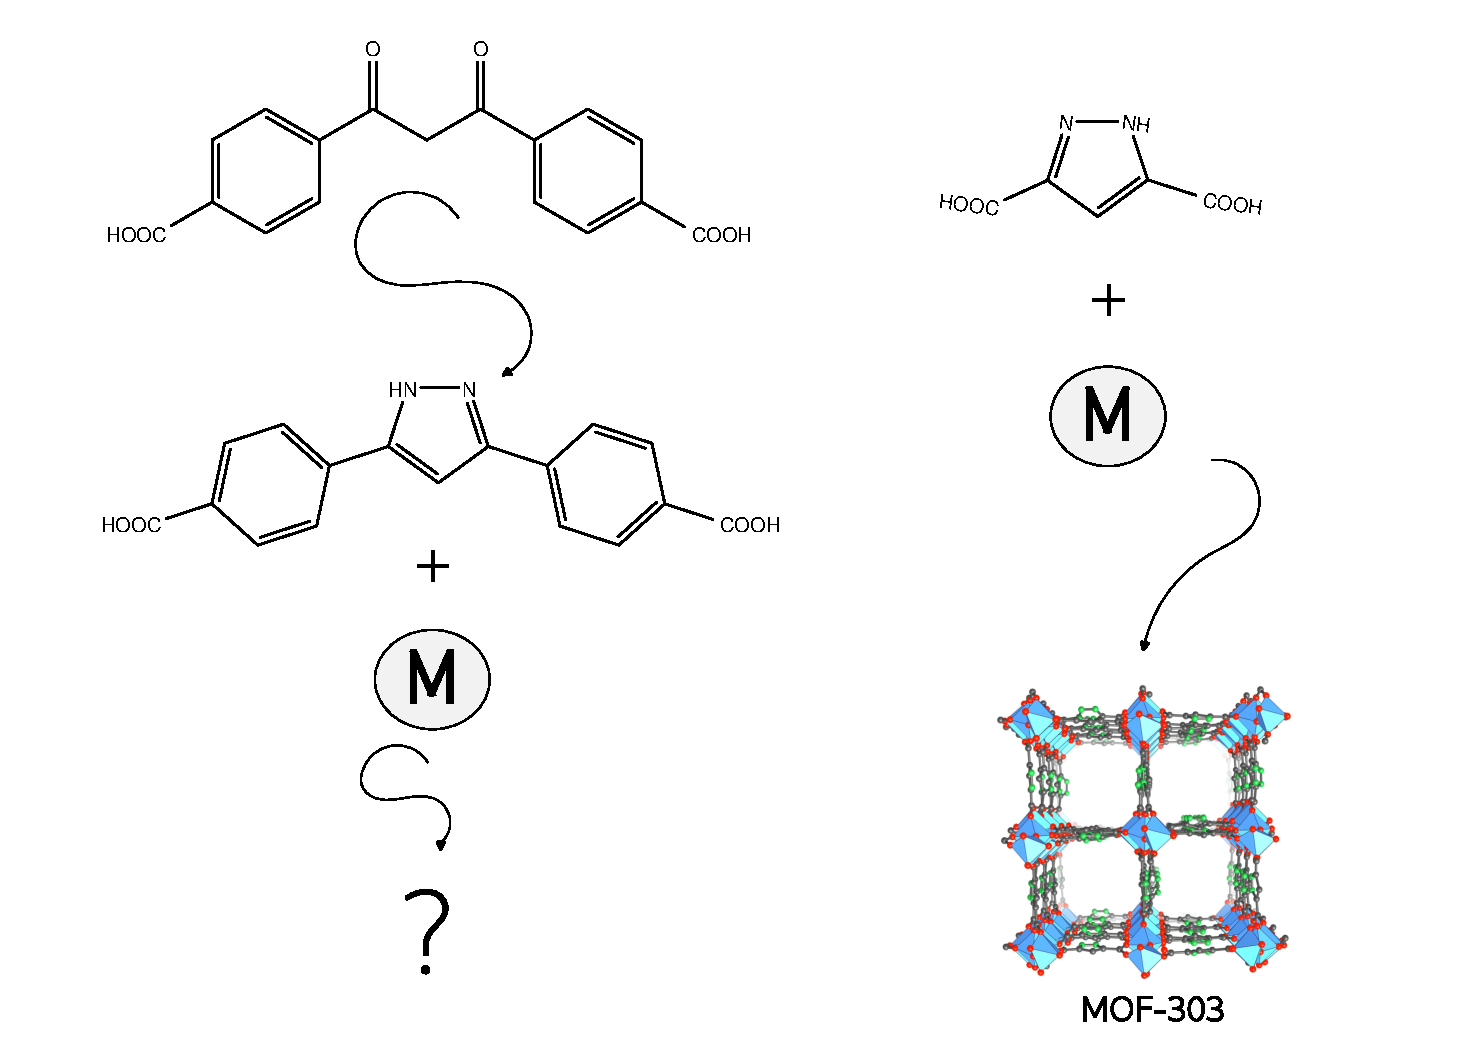
\includegraphics[width=8cm,keepaspectratio]{illustration/drawing2.pdf}
			\end{figure}
		\end{column}
	\end{columns}
\end{frame}

\subsection{Addizione diretta di idrazina al dichetone}
\begin{frame}{Addizione diretta di idrazina al dichetone}
	\framesubtitle{Retrosintesi}
	\begin{figure}[h]
		\centering
		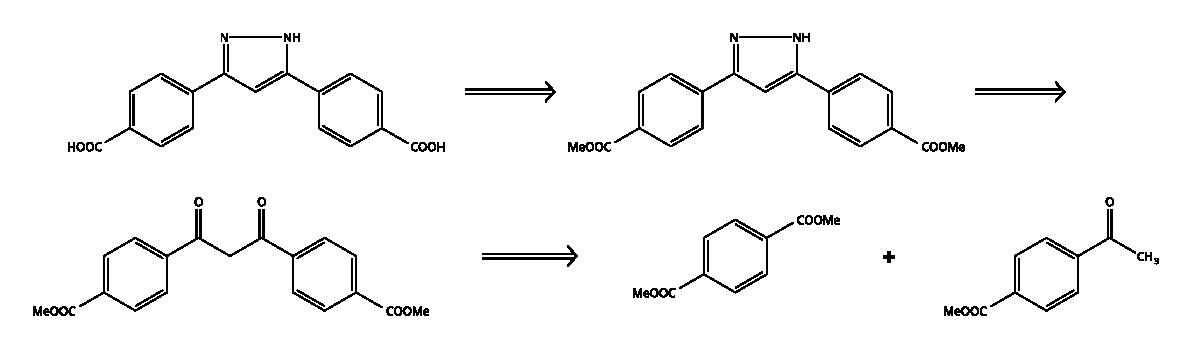
\includegraphics[width=14cm,height=8cm,keepaspectratio]{../Structures/pyr-retro.eps}
		\caption{Approccio retrosintetico sfruttando l'addizione diretta di idrazina}
	\end{figure}
\end{frame}

% TODO: aggiungere NMR e/o IR, almeno da avere qualche informazione sulla caratterizzazione
\begin{frame}{Addizione diretta di idrazina al dichetone}
	\framesubtitle{Valutazione dell'efficacia dei passaggi sintetici}
	\begin{figure}[h]
		\centering
		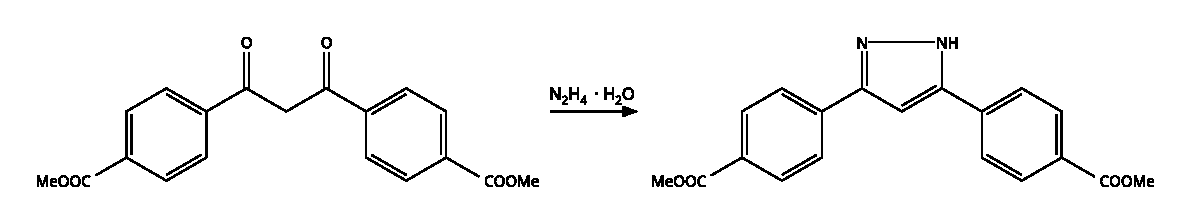
\includegraphics[width=10cm,height=8cm,keepaspectratio]{../Structures/pyrazole-form.eps}
		\caption{Reazione chiave di formazione dell'anello pirazolico}
	\end{figure}
	\begin{footnotesize}
		\begin{center}
			\begin{tabular}{cc}
				\toprule
				{Reazione}                                    & Resa [\%]     \\
				\midrule
				Claisen mista per la formazione del dichetone & \(92\)        \\
				Addizione di idrazina al dichetone            & \(< 25\)      \\
				Idrolisi                                      & \(\simeq 70\) \\
				\bottomrule
			\end{tabular}
		\end{center}
	\end{footnotesize}
\end{frame}

\begin{frame}{Addizione diretta di idrazina al dichetone}
	\framesubtitle{Condizioni di Reazione e Recupero del Prodotto}
	\begin{columns}
		\hspace{1cm}
		\begin{column}{0.5\textwidth}
			Condizioni di reazione
			\begin{itemize}
				\item Solvente e solubilitá
				\item Temperatura
				\item Tempo di reazione
			\end{itemize}
			\vspace{0.2cm}
			Recupero del prodotto
			\begin{itemize}
				\item Ricristallizzazione
				\item Colonna Cromatografica
				\item Soxhlet
			\end{itemize}
		\end{column}
		\hspace{-3cm}
		\begin{column}{0.5\textwidth}
			\vspace{-0.5cm}
			\begin{figure}[h!]
				\centering
				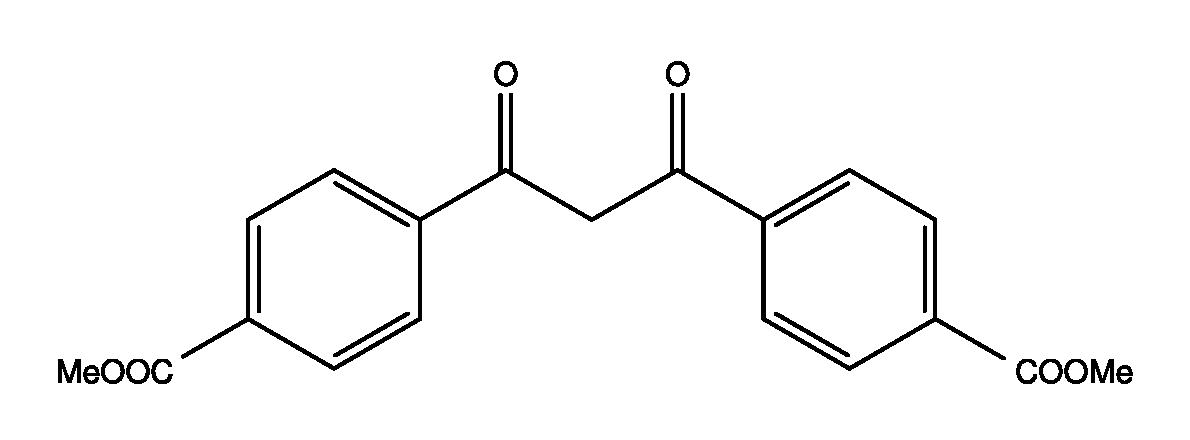
\includegraphics[width=5cm,height=5cm,keepaspectratio]{../Structures/dikest2.eps}
				\caption{Struttura dell'intermedio di partenza}
			\end{figure}
			\begin{footnotesize}
				\begin{center}
					\begin{tabular}{ccc}
						\toprule
						{Solvente} & T [K] & Resa [\%]     \\
						\midrule
						DMF        & 403   & \(< 10\)      \\
						DMSO       & 433   & \(\simeq 25\) \\
						EtOH       & 351   & \(< 5\)       \\
						THF        & 339   & \(< 5\)       \\
						\bottomrule
					\end{tabular}
				\end{center}
			\end{footnotesize}
		\end{column}
	\end{columns}
\end{frame}

\subsection{Addizione coniugata di idrazina all'alfabeta insaturo}

\begin{frame}{Addizione coniugata di idrazina all'alfabeta insaturo}
	\framesubtitle{Retrosintesi}
	\begin{figure}[h!]
		\centering
		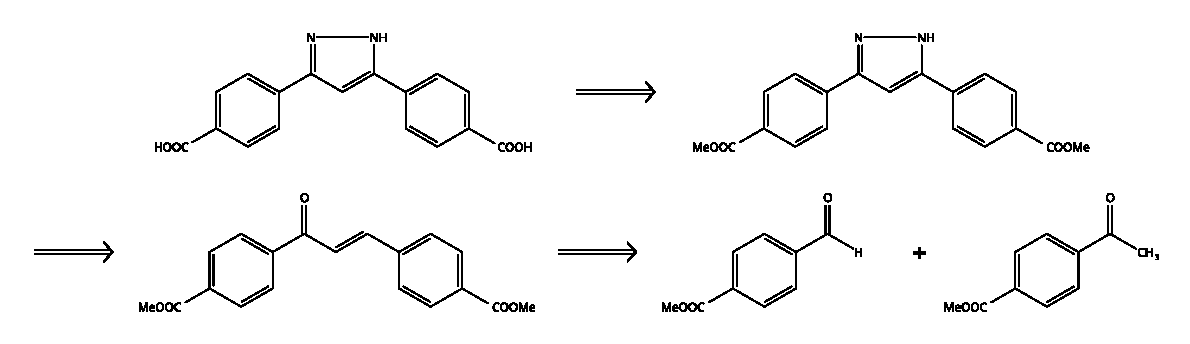
\includegraphics[width=13cm,height=8cm,keepaspectratio]{../Structures/pyrazole-retro-alt.eps}
		\caption{Approccio retrosintetico sfruttando l'addizione coniugata di idrazina}
	\end{figure}
\end{frame}

% TODO: aggiungere NMR e/o IR, almeno da avere qualche informazione sulla caratterizzazione
\begin{frame}{Addizione coniugata di idrazina all'alfabeta insaturo}
	\framesubtitle{Valutazione dell'efficacia dei passaggi sintetici}
	\begin{figure}[h]
		\centering
		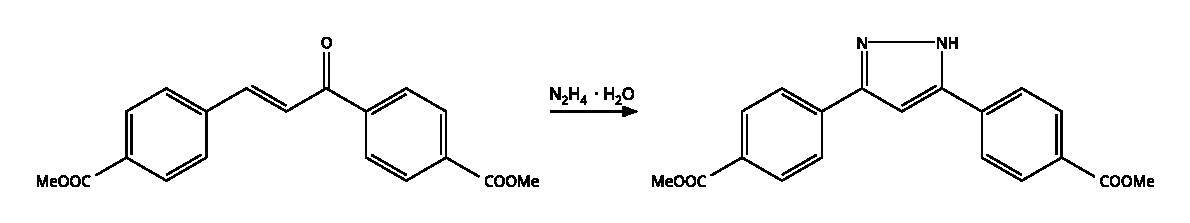
\includegraphics[width=10cm,height=8cm,keepaspectratio]{../Structures/pyrazole-form-alt.eps}
		\caption{Reazione chiave di formazione dell'anello pirazolico}
	\end{figure}
	\begin{footnotesize}
		\begin{center}
			\begin{tabular}{cc}
				\toprule
				{Reazione}                                                                & Resa [\%]     \\
				\midrule
				Condensazione crotonica per la formazione dell'\(\alpha,\beta \)-insaturo & \(94\)        \\
				Addizione di idrazina al \(\alpha,\beta \)-insaturo                       & \(< 25\)      \\
				Idrolisi                                                                  & \(\simeq 70\) \\
				\bottomrule
			\end{tabular}
		\end{center}
	\end{footnotesize}
\end{frame}

\begin{frame}{Addizione diretta di idrazina al dichetone}
	\framesubtitle{Condizioni di Reazione e Recupero del Prodotto}
	\begin{columns}
		\hspace{1cm}
		\begin{column}{0.5\textwidth}
			Condizioni di reazione
			\begin{itemize}
				\item Solvente e solubilitá
				\item Catalisi acida e basica
				\item Temperatura
				\item Tempo di reazione
				\item Microonde
			\end{itemize}
		\end{column}
		\hspace{-3cm}
		\begin{column}{0.5\textwidth}
			\vspace{-0.5cm}
			\begin{figure}[h!]
				\centering
				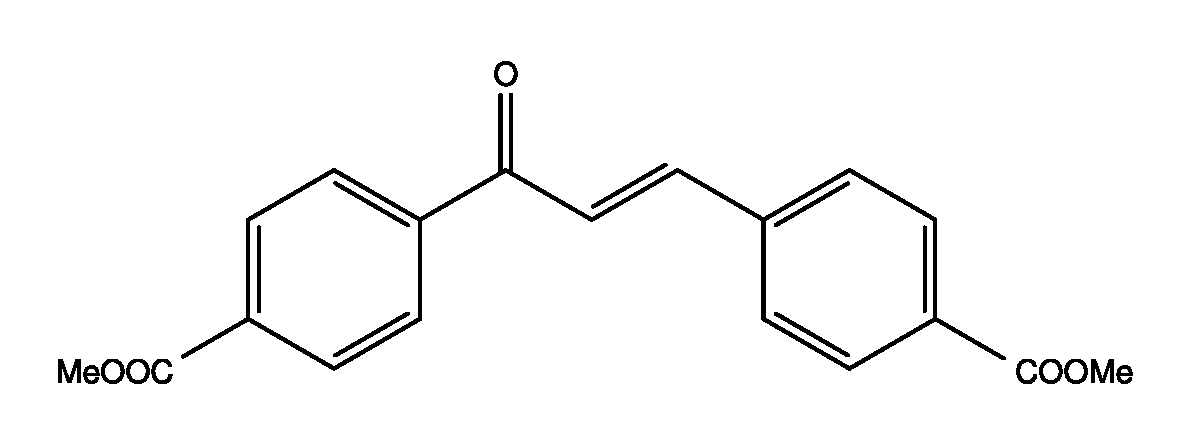
\includegraphics[width=5cm,height=5cm,keepaspectratio]{../Structures/unsaturated.eps}
				\caption{Struttura dell'intermedio di partenza}
			\end{figure}
			\begin{footnotesize}
				\begin{center}
					\begin{tabular}{ccc}
						\toprule
						{Solvente} & T [K]   & Resa [\%] \\
						\midrule
						AcOH       & \(391\) & \(< 5\)   \\
						EtOH + HCl & \(351\) & \(< 5\)   \\
						EtOH + Py  & \(351\) & \(< 5\)   \\
						\bottomrule
					\end{tabular}
				\end{center}
			\end{footnotesize}
		\end{column}
	\end{columns}
\end{frame}

% TODO: Aggiungere struttura del sottoprodotto idrazonico
\begin{frame}{Addizione diretta di idrazina al dichetone}
	\framesubtitle{Intermedio idrazonico}

	\begin{figure}[h!]
		\centering
		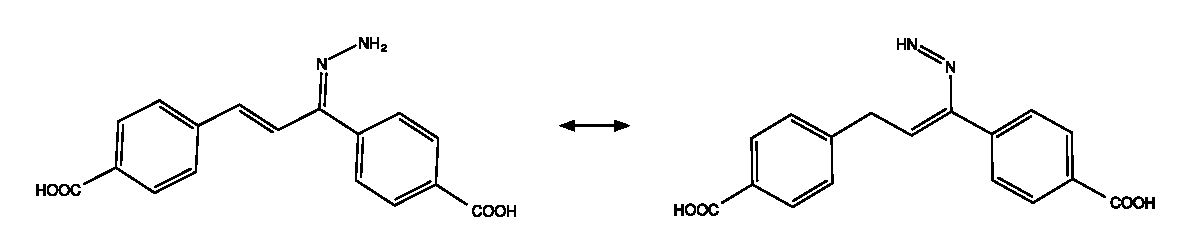
\includegraphics[width=10cm,keepaspectratio]{../Structures/idrazone.eps}
		\caption{Risonanza dell'intermedio idrazonico}
	\end{figure}


\end{frame}

\section{Caratterizzazione elettrochimica di leganti dichetonici}

\begin{frame}{Perché elettrochimica?}
	\begin{columns}
		\begin{column}{0.5\textwidth}
			\begin{itemize}
				\item Valutazione della reattivitá elettrochimica
				\item Determinazione delle proprietá elettroniche
				\item Relazione con le transizioni elettroniche osservate in spettroscopia
			\end{itemize}
		\end{column}
		\begin{column}{0.5\textwidth}
			\begin{center}
				\begin{itemize}
					\begin{figure}[h!]
						\hspace{-1cm}
						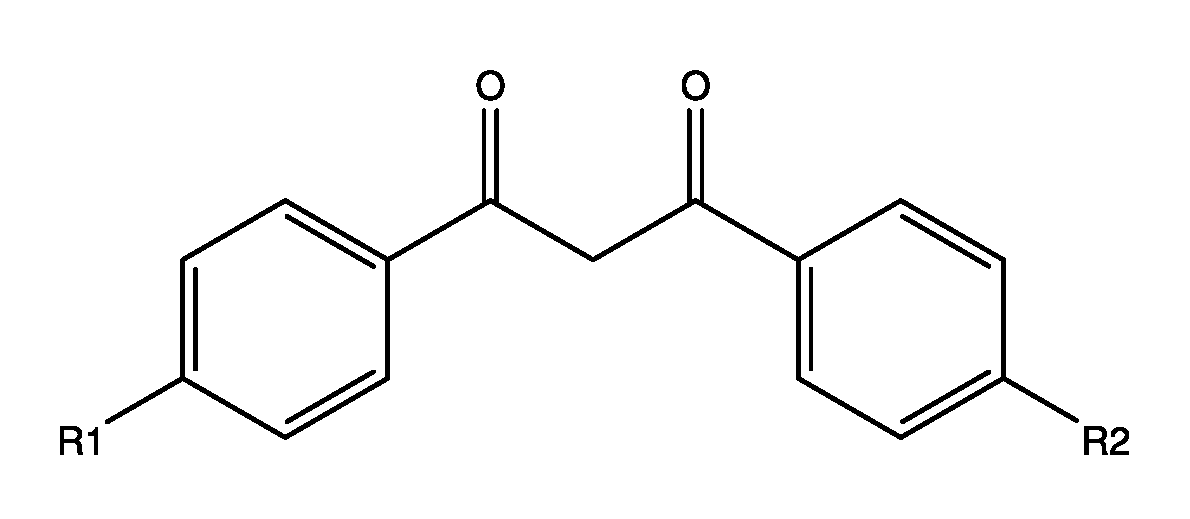
\includegraphics[width=6cm,keepaspectratio]{../Structures/electrochemistry-generic.eps}
						\caption{Struttura generica di un legante dichetonico}
					\end{figure}
				\end{itemize}
			\end{center}
		\end{column}
	\end{columns}
\end{frame}

\begin{frame}{Caratterizzazione UV}
	\vspace{-0.5cm}
	\begin{columns}
		\hspace{-1cm}
		\begin{column}{0.5\textwidth}
			\begin{figure}[h!]
				\centering
				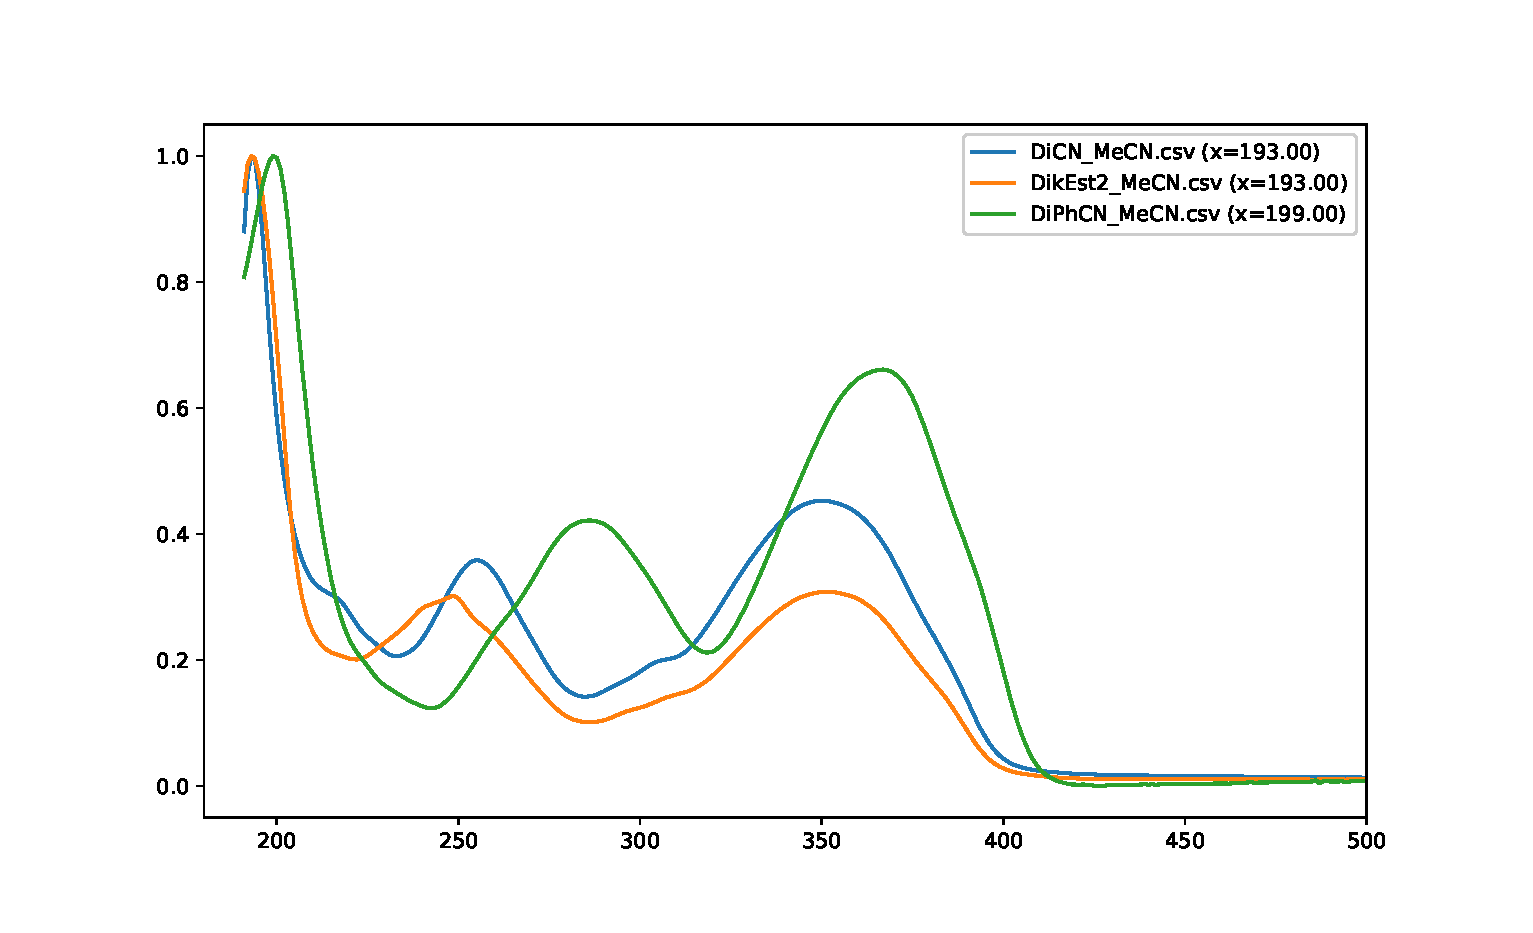
\includegraphics[width=8cm,keepaspectratio]{../Spectra/LegantiMeCN.eps}
				\vspace*{-8mm}
				\hspace*{3cm}
				\caption{UV in MeCN}
			\end{figure}
		\end{column}
		\hspace{-0.5cm}
		\begin{column}{0.5\textwidth}
			\begin{figure}[h!]
				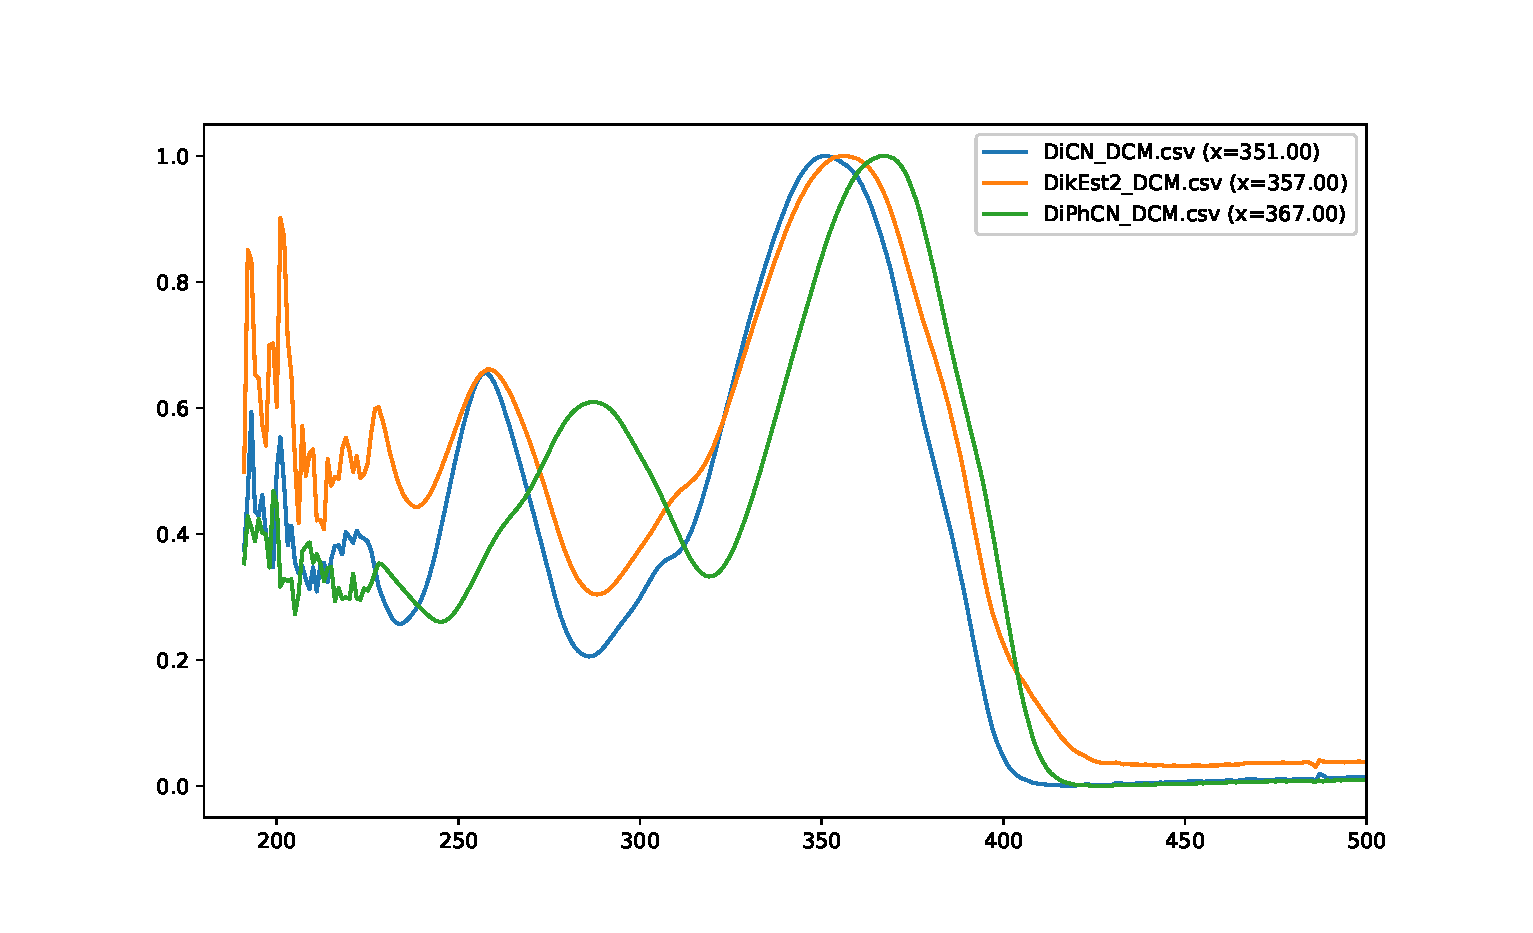
\includegraphics[width=8cm,keepaspectratio]{../Spectra/LegantiDCM.eps}
				\vspace*{-8mm}
				\caption{UV in MeCN}
			\end{figure}
		\end{column}
	\end{columns}
\end{frame}

\backmatter
\end{document}
